\documentclass{article}
\usepackage[utf8]{inputenc}
\usepackage{longtable}
\usepackage{gensymb}
\usepackage{graphicx}
\usepackage{siunitx}
\usepackage{caption}
\usepackage[colorlinks,bookmarks=false,citecolor=blue,linkcolor=blue,urlcolor=blue]{hyperref}
\usepackage{relsize}
\usepackage{amsmath}
\usepackage{booktabs}
\usepackage{amssymb}
\usepackage{bm}
\usepackage{multirow}
\usepackage{placeins}
\begin{document}
\begin{titlepage}
\begin{center}

\includegraphics[scale=0.12]{document/niser.png}
\line(1,0){345}\\
[1mm]
\begin{large}
\textbf{\LARGE Diffraction of Light due to \\ \huge Ultrasonic Wave Propagation in Liquids}\\ 
\end{large}
\line(1,0){240}\\
[5cm]
\large MAITREY SHARMA\\
\small (1911093)\\
[3.5cm]
Third Year Integrated M.Sc.\\
\textbf{School of Physical Sciences}\\
\textbf{National Institute of Science Education and Research, Bhubaneshwar}\\
\small October 26, 2021
\end{center} 
\end{titlepage}
\newpage
\section{Aim}
\begin{itemize}
    \item To study the diffraction of light due to propagation of ultrasonic wave in a liquid
    \item To determine the speed of sound in various liquids at room temperature
    \item To determine the compressibility of the given liquids.
\end{itemize}

\section{Apparatus}
\begin{itemize}
    \item Radio frequency oscillator fitted with a frequency meter,
    \item Quartz crystal slab fitted with two leads,
    \item Spectrometer,
    \item A glass cell with sample liquid (kerosene/toluene/turpentine oil etc),
    \item A sodium lamp and a spirit level
\end{itemize}

\section{Introduction}
\noindent
\textbf{Acoustic waves} are a type of energy propagation through a medium by means of adiabatic compression and decompression. Acoustic waves travel with a characteristic acoustic velocity that depends on the medium they're passing through. Some examples of acoustic waves are audible sound from a speaker (waves traveling through air at the speed of sound), ground movement from an earthquake (waves traveling through the earth), or ultrasound used for medical imaging (waves traveling through the body).
\par
\noindent
Acoustic waves in liquids cause density changes with spacing determined by the 
frequency and the speed of the sound wave. For ultrasonic waves with frequencies in the $\si{\mega \hertz}$ range, the spacing between the high and low density regions are similar to the spacing used in diffraction gratings. Since these density changes in liquids will cause changes in the index of refraction of the liquid, it can be shown that parallel light passed through the excited liquid will be diffracted much as if it had passed through a grating. The experiment can serve as an indirect method of measuring the velocity of sound in various liquids. The phenomenon of interaction between light and sound waves in a liquid is called the \textbf{Debye-Sears effect} after they first observed the phenomena of diffraction of light using an ultrasonic grating in 1932.
\par
\noindent
An ultrasonic grating is a type of diffraction grating produced by interfering ultrasonic waves in a medium altering the physical properties of the medium, and hence the refractive index, in a grid-like pattern. The term acoustic grating is a more general term that includes operation at audible frequencies.
\par
\noindent
An ultrasonic wave is a sound wave at a frequency greater than $\SI{20}{\kilo \hertz}$. The human ear cannot recognize ultrasonic waves. Ultrasonic waves can be produced by the piezoelectric effect (the phenomena of generation of emf due to mechanical stress in some solids) and magnetostriction (a property of magnetic materials that causes them to change their shape or dimensions during the process of magnetization. It is caused by  energy loss due to frictional heating in susceptible ferromagnetic cores.).


\section{Schematic}

\begin{figure}[hbt!]
    \centering
    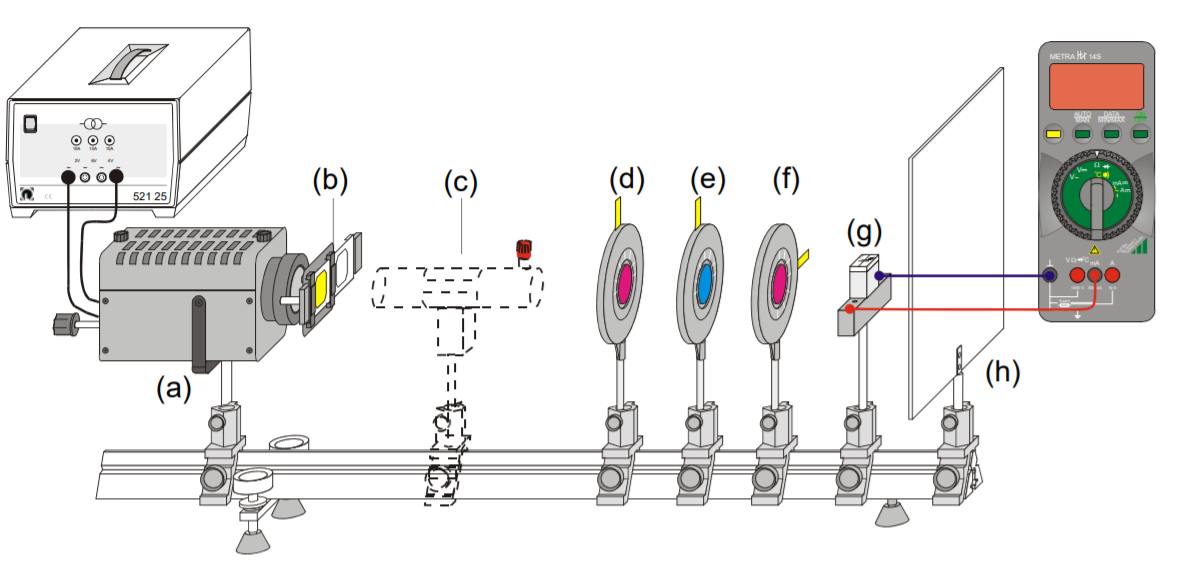
\includegraphics[scale = 0.65]{Figures/schematic.png}
    \captionsetup{justification=centering}
    \caption{The schematic of the ultrasonic diffraction experiment }
    \label{fig:schematic}
\end{figure}



\section{Theory}
\noindent 
Diffraction phenomenon similar to those with ordinary ruled grating is observed 
when ultrasonic waves traverse through a liquid. The ultrasonic waves passing through 
a liquid is an elastic wave in which compressions (region of increased density in the medium as the disturbance travels) and rarefactions (region of reduced density in the medium as the disturbance travels) travel one behind the other spaced regularly apart. The successive separations between two compressions or rarefactions are equal to the wavelength of ultrasonic wave, $\lambda_u$ in the liquid. Due to reflections at the sides of the tank or the container, a stationary wave pattern is obtained 
with nodes (the locations at which the absolute value of the amplitude is minimum) and anti-nodes (the locations where the absolute value of the amplitude is maximum) at regular intervals. We are thus dealing and hence having a periodically changing index of rarefactions which produces diffraction of light according to the grating rule.
\par
\noindent
If $\lambda_u$ denotes the wavelength of sound in the liquid, $\lambda$ the wavelength of incident light in air and $\theta_n$ is angle of diffraction of n\textsuperscript{th} order, then we have,
\begin{equation}
    d \sin \theta_n = n \lambda
\end{equation}
In a transparent medium, variations in density correspond to variations in the index of 
refraction and therefore a monochromatic parallel light beam traveling perpendicular to 
the sound direction is refracted as if it had passed through a diffraction grating of spacing $d = \lambda_u$, thus
\begin{equation}
    \lambda_u \sin \theta_n = n \lambda
\end{equation}
If $\nu$ is the frequency of the crystal, the velocity $V_u$ of ultrasonic wave in the 
liquid is given by,
\begin{equation}
    V_u = \nu \lambda_u
\end{equation}
Thus, by measuring the angle of diffraction $\theta_n$, the order of diffraction $n$, the wavelength of light, the wavelength of ultrasonic wave in the liquid can be determined and then knowing the frequency of sound wave, its velocity $V_u$ can be obtained.
\par
\noindent
The speed of sound depends on both an inertial property of the medium (to store kinetic 
energy) and an elastic property (to store potential energy):
\begin{equation}
    V_u = \sqrt{\dfrac{\text{elastic property}}{\text{inertial property}}}
\end{equation}
For a liquid medium, the bulk modulus $B$ accounts for the extent to which an element 
from the medium changes in volume when a pressure is applied:
\begin{equation}
    B = - \dfrac{\Delta P}{\dfrac{\Delta V}{V}}
\end{equation}
Here $\dfrac{\Delta V}{V}$ is the fractional change in volume produced by change in pressure $\Delta P$. The sign of $\Delta V$ and $\Delta P$ are always opposite. The unit of $B$ is Pascal ($\si{\pascal}$). Therefore, the speed of sound in liquid can be expressed as
\begin{equation}
\label{eq6}
    V_u = \dfrac{\nu \lambda n}{\sin \theta} = \sqrt{\dfrac{B}{\rho}}
\end{equation}
Thus,
\begin{equation}
\label{eq7}
    B = V_u^2 \rho = \dfrac{1}{K}
\end{equation}
where $B$ is the bulk modulus of elasticity, $\rho$ is the density of the liquid and $K$ is the compressibility of liquid.

\section{Observations and Results}
\begin{enumerate}
    \item Density of turpentine, $\rho_1 = \SI{865}{\kilogram \per \metre \cubed}$
    \item Frequency of vibrating crystal used, $\nu_1 = \SI{3.9911}{\mega \hertz}$
    \item Density of toluene, $\rho_2 = \SI{867}{\kilogram \per \metre \cubed}$
    \item Frequency of vibrating crystal used, $\nu_2 = \SI{4.2633}{\mega \hertz}$
\end{enumerate}


% Please add the following required packages to your document preamble:
% \usepackage{booktabs}
% \usepackage{multirow}

\begin{table}[]
\centering
\caption{\label{tab:tur}Readings for the experiment using Turpentine}
\resizebox{\textwidth}{!}{%
\begin{tabular}{@{}cccccccccc@{}}
\toprule
\multicolumn{2}{c}{\multirow{2}{*}{\textbf{Order}}} &
  \multicolumn{2}{c}{\begin{tabular}[c]{@{}c@{}}\textbf{Left}\\ \textbf{of center}\end{tabular}} &
  \multicolumn{2}{c}{\begin{tabular}[c]{@{}c@{}}\textbf{Right}\\ \textbf{of center}\end{tabular}} &
  \begin{tabular}[c]{@{}c@{}}\bm{2$\theta$}\\ ($a-b$)\end{tabular} &
  \begin{tabular}[c]{@{}c@{}}\bm{2$\theta$}\\ ($a'-b'$)\end{tabular} &
  \begin{tabular}[c]{@{}c@{}}\textbf{Average}\\ \bm{2$\theta$}\end{tabular} &
  \bm{$\theta$} \\
\multicolumn{2}{c}{} &
  $a$ &
  $a'$ &
  $b$ &
  $b'$ &
  (deg) &
  (deg) &
  (deg) &
  (deg) \\ \midrule
\multirow{2}{*}{\begin{tabular}[c]{@{}c@{}}\textbf{Set}\\ \textbf{I}\end{tabular}} &
  \begin{tabular}[c]{@{}c@{}}\textit{First}\\ \textit{Order}\end{tabular} &
  \begin{tabular}[c]{@{}c@{}}106\\ 47/60\end{tabular} &
  \begin{tabular}[c]{@{}c@{}}286\\ 8/15\end{tabular} &
  \begin{tabular}[c]{@{}c@{}}106\\ 29/30\end{tabular} &
  \begin{tabular}[c]{@{}c@{}}286\\ 43/60\end{tabular} &
  11/60 &
  11/60 &
  11/60 &
  11/120 \\ \cmidrule(l){2-10} 
 &
  \begin{tabular}[c]{@{}c@{}}\textit{Second}\\ \textit{Order}\end{tabular} &
  \begin{tabular}[c]{@{}c@{}}106\\ 19/30\end{tabular} &
  \begin{tabular}[c]{@{}c@{}}286\\ 13/30\end{tabular} &
  \begin{tabular}[c]{@{}c@{}}107\\ 1/15\end{tabular} &
  \begin{tabular}[c]{@{}c@{}}286\\ 9/10\end{tabular} &
  13/30 &
  7/15 &
  9/20 &
  9/40 \\ \midrule
\multirow{2}{*}{\begin{tabular}[c]{@{}c@{}}\textbf{Set}\\ \textbf{II}\end{tabular}} &
  \begin{tabular}[c]{@{}c@{}}\textit{First}\\ \textit{Order}\end{tabular} &
  \begin{tabular}[c]{@{}c@{}}106\\ 3/4\end{tabular} &
  \begin{tabular}[c]{@{}c@{}}286\\ 8/15\end{tabular} &
  \begin{tabular}[c]{@{}c@{}}106\\ 29/30\end{tabular} &
  \begin{tabular}[c]{@{}c@{}}286\\ 3/4\end{tabular} &
  13/60 &
  13/60 &
  13/60 &
  13/120 \\ \cmidrule(l){2-10} 
 &
  \begin{tabular}[c]{@{}c@{}}\textit{Second}\\ \textit{Order}\end{tabular} &
  \begin{tabular}[c]{@{}c@{}}106\\ 13/20\end{tabular} &
  \begin{tabular}[c]{@{}c@{}}286\\ 9/20\end{tabular} &
  \begin{tabular}[c]{@{}c@{}}107\\ 1/20\end{tabular} &
  \begin{tabular}[c]{@{}c@{}}286\\ 47/60\end{tabular} &
  2/5 &
  1/3 &
  11/30 &
  11/60 \\ \bottomrule
\end{tabular}%
}
\end{table}

\begin{table}[]
\small
\centering
\caption{\label{tab:vtur}Velocities as calculated from table (\ref{tab:tur})}
\begin{tabular}{@{}cccc@{}}
\toprule
\multirow{2}{*}{\textbf{Order}}                                & \multicolumn{2}{c}{\bm{$V_u$}} & \multirow{2}{*}{\begin{tabular}[c]{@{}c@{}}\textbf{Average}\\ \bm{$V_u$}\end{tabular}} \\
                                                       & \textbf{Set I}      & \textbf{Set II}     &  \\ \midrule
\begin{tabular}[c]{@{}c@{}}\textit{First}\\ \textit{Order}\end{tabular} & 1470.0782  & 1243.9125 & \multirow{2}{*}{1345.4787}                                         \\
\begin{tabular}[c]{@{}c@{}}\textit{Second}\\ \textit{Order}\end{tabular} & 1197.8440 & 1470.0801 &  \\ \bottomrule
\end{tabular}
\end{table}






\begin{table}[]
\centering
\caption{\label{tab:tol}Readings for the experiment using Toluene}
\resizebox{\textwidth}{!}{%
\begin{tabular}{@{}cccccccccc@{}}
\toprule
\multicolumn{2}{c}{\multirow{2}{*}{\textbf{Order}}} &
  \multicolumn{2}{c}{\begin{tabular}[c]{@{}c@{}}\textbf{Left}\\ \textbf{of center}\end{tabular}} &
  \multicolumn{2}{c}{\begin{tabular}[c]{@{}c@{}}\textbf{Right}\\ \textbf{of center}\end{tabular}} &
  \begin{tabular}[c]{@{}c@{}}\bm{2$\theta$}\\ ($a-b$)\end{tabular} &
  \begin{tabular}[c]{@{}c@{}}\bm{2$\theta$}\\ ($a'-b'$)\end{tabular} &
  \begin{tabular}[c]{@{}c@{}}\textbf{Average}\\ \bm{2$\theta$}\end{tabular} &
  \bm{$\theta$} \\
\multicolumn{2}{c}{} &
  $a$ &
  $a'$ &
  $b$ &
  $b'$ &
  (deg) &
  (deg) &
  (deg) &
  (deg) \\ \midrule
\multirow{2}{*}{\begin{tabular}[c]{@{}c@{}}\textbf{Set}\\ \textbf{I}\end{tabular}} &
  \begin{tabular}[c]{@{}c@{}}\textit{First}\\ \textit{Order}\end{tabular} &
  \begin{tabular}[c]{@{}c@{}}107\\ 1/12\end{tabular} &
  \begin{tabular}[c]{@{}c@{}}286\\ 9/10\end{tabular} &
  \begin{tabular}[c]{@{}c@{}}107\\ 4/15\end{tabular} &
  \begin{tabular}[c]{@{}c@{}}287\\ 1/12\end{tabular} &
  11/60 &
  11/60 &
  11/60 &
  11/120 \\ \cmidrule(l){2-10} 
 &
  \begin{tabular}[c]{@{}c@{}}\textit{Second}\\ \textit{Order}\end{tabular} &
  \begin{tabular}[c]{@{}c@{}}106\\ 29/30\end{tabular} &
  \begin{tabular}[c]{@{}c@{}}286\\ 47/60\end{tabular} &
  \begin{tabular}[c]{@{}c@{}}107\\ 23/60\end{tabular} &
  \begin{tabular}[c]{@{}c@{}}287\\ 1/6\end{tabular} &
  5/12 &
  23/60 &
  2/5 &
  1/5 \\ \midrule
\multirow{2}{*}{\begin{tabular}[c]{@{}c@{}}\textbf{Set}\\ \textbf{II}\end{tabular}} &
  \begin{tabular}[c]{@{}c@{}}\textit{First}\\ \textit{Order}\end{tabular} &
  \begin{tabular}[c]{@{}c@{}}107\\ 1/15\end{tabular} &
  \begin{tabular}[c]{@{}c@{}}286\\ 5/6\end{tabular} &
  \begin{tabular}[c]{@{}c@{}}107\\ 17/60\end{tabular} &
  \begin{tabular}[c]{@{}c@{}}287\\ 1/12\end{tabular} &
  13/60 &
  1/4 &
  7/30 &
  7/60 \\ \cmidrule(l){2-10} 
 &
  \begin{tabular}[c]{@{}c@{}}\textit{Second}\\ \textit{Order}\end{tabular} &
  \begin{tabular}[c]{@{}c@{}}106\\ 19/20\end{tabular} &
  \begin{tabular}[c]{@{}c@{}}286\\ 47/60\end{tabular} &
  \begin{tabular}[c]{@{}c@{}}107\\ 2/5\end{tabular} &
  \begin{tabular}[c]{@{}c@{}}287\\ 1/5\end{tabular} &
  9/20 &
  5/12 &
  13/30 &
  13/60 \\ \bottomrule
\end{tabular}%
}
\end{table}

\begin{table}[]
\small
\centering
\caption{\label{tab:vtol}Velocities as calculated from table (\ref{tab:tol})}
\begin{tabular}{@{}cccc@{}}
\toprule
\multirow{2}{*}{\textbf{Order}}                                & \multicolumn{2}{c}{\bm{$V_u$}} & \multirow{2}{*}{\begin{tabular}[c]{@{}c@{}}\textbf{Average}\\ \bm{$V_u$}\end{tabular}} \\
                                                       & \textbf{Set I}      & \textbf{Set II}     &  \\ \midrule
\begin{tabular}[c]{@{}c@{}}\textit{First}\\ \textit{Order}\end{tabular} & 1570.3401  & 1233.8390 & \multirow{2}{*}{1393.1029}                                         \\
\begin{tabular}[c]{@{}c@{}}\textit{Second}\\ \textit{Order}\end{tabular} & 1439.4807 & 1328.7519 &  \\ \bottomrule
\end{tabular}
\end{table}


\section{Results}
From table (\ref{tab:vtur}), we have velocity of ultrasonic wave in turpentine as $V_u^{(1)} = \SI{1345.4787}{\metre \per \second}$ and from table (\ref{tab:vtol}), the velocity of ultrasonic wave in toluene is $V_u^{(2)} = \SI{1393.1029}{\metre \per \second}$. From this we can calculate the bulk modulus of elasticity of the liquids using equation (\ref{eq7}). Therefore, we have the bulk modulus of turpentine,
\begin{equation}
    \boxed{B_1 = \SI{1.6e9}{\pascal}}
\end{equation}
and the bulk modulus of toluene,
\begin{equation}
    \boxed{B_2 = \SI{1.7e9}{\pascal}}
\end{equation}


\section{Error Analysis}
\subsection{Relative Errors}
The observed velocity in turpentine is $V_u^{(1)} = \SI{1345.4787}{\metre \per \second}$ whereas the expected velocity was $\SI{1240}{\metre \per \second}$. Thus, relative error in velocity in turpentine is
\begin{equation}
    \delta = \biggl| \dfrac{1345.4787-1240}{1240} \biggr| \times 100 \% \approx 8.5 \%
\end{equation}
In the same way, the observed velocity in toluene is $V_u^{(2)} = \SI{1393.1029}{\metre \per \second}$ whereas the expected velocity was $\SI{1306}{\metre \per \second}$. Thus, relative error in velocity in toluene is
\begin{equation}
    \delta = \biggl| \dfrac{1393.1029-1306}{1306} \biggr| \times 100 \% \approx 6.7 \%
\end{equation}
Now, the observed value of bulk modulus of elasticity of turpentine is $B_1 = \SI{1.58e9}{\pascal}$ whereas the expected value was $\SI{1.28e9}{\pascal}$. Thus, relative error in value of bulk modulus of elasticity of turpentine is
\begin{equation}
   \delta = \biggl| \dfrac{(1.58 - 1.28) \times 10^9}{1.28 \times 10^9} \biggr| \times 100 \% \approx 23.4 \% 
\end{equation}
In the same way, the observed value of bulk modulus of elasticity of toluene is $B_2 = \SI{1.70e9}{\pascal}$ whereas the expected value was $\SI{1.09e9}{\pascal}$. Thus, relative error in value of bulk modulus of elasticity of toluene is
\begin{equation}
    \delta = \biggl| \dfrac{(1.70 - 1.09) \times 10^9}{1.09 \times 10^9} \biggr| \times 100 \% \approx 56.0 \% 
\end{equation}
\subsection{Propagational Errors}
The propagational error in the velocity of ultrasonic wave will be given by
\begin{equation}
\label{eq14}
    d V_u = \sqrt{\Bigg( \dfrac{\partial V_u}{\partial \nu} \cdot\sigma_{\nu}\Bigg)^2 + \Bigg( \dfrac{\partial V_u}{\partial (\sin \theta)} \cdot \sigma_{\sin \theta} \Bigg)^2} 
\end{equation}
For this we first need to find error in $\sin \theta$. Error in $\sin \theta$ will come from the uncertainty in the measurement of $\theta$ (in radians), which is equal to $\sigma_{\theta} = \SI{2.9e-4}{\radian}$. Now error in $\sin \theta$ is given by
\begin{equation}
\label{eq15}
    \sigma_{\sin \theta} = (\cos \theta) \cdot \sigma_{\theta}
\end{equation}
We calculate error for each reading individually using equation (\ref{eq15}) and (\ref{eq14}) and we will then take the \textit{average} of the obtained errors. After doing the calculations, we obtain for turpentine, 
\begin{equation}
    \boxed{d V_u^{(1)} \approx \SI{170}{\metre \per \second}}
\end{equation}
Note that, $\sigma_{\nu}$ is the uncertainty in the value of frequency of crystal and is taken to be $\SI{0.0001}{\mega \hertz}$ and $V_u$ is given by equation (\ref{eq6}).
\par
\noindent
Similarly for toluene, the uncertainty in velocity of ultrasonic wave is given by
\begin{equation}
    \boxed{d V_u^{(2)} \approx \SI{170}{\metre \per \second}}
\end{equation}
\par
\noindent
Now the propagation error in bulk modulus is given by
\begin{equation}
    d B = \sqrt{\Bigg(\dfrac{\partial B}{\partial V_u} \cdot \sigma_{V_u} \Bigg)^2}
\end{equation}
$\sigma_{V_u}$ is the uncertainty in $V_u$, that is $d V_u$, and we have already calculated it to be $\SI{170}{\metre \per \second}$. Therefore putting in the values, for turpentine, we get
\begin{equation}
    \boxed{d B_1 \approx \SI{0.4e9}{\pascal}}
\end{equation}
and for toluene, 
\begin{equation}
    \boxed{d B_2 \approx \SI{0.4e9}{\pascal}}
\end{equation}

\section{Conclusions and Discussions}
\begin{enumerate}
    \item The velocity of ultrasonic acoustic waves through turpentine was found to be $V_u^{(1)} = \SI[separate-uncertainty=true]{1345 \pm 170}{\metre \per \second}$ after taking care of significant figures. The observed velocity was found to be close to the literature value.
    \item The velocity of ultrasonic acoustic waves through toluene was found to be $V_u^{(2)} = \SI[separate-uncertainty=true]{1393 \pm 170}{\metre \per \second}$ after taking care of significant figures. The observed velocity was found to be close to the literature value.
    \item The bulk modulus of elasticity of turpentine was found to be \\ $B_1 = \SI[separate-uncertainty=true]{1.6 \pm 0.4}{\giga \pascal}$ after taking care of significant figures. The observed bulk modulus of elasticity was found to be close enough to the literature value. 
    \item The bulk modulus of elasticity of toluene was found to be \\
    $B_2 = \SI[separate-uncertainty=true]{1.7 \pm 0.4}{\giga \pascal}$ after taking care of significant figures. The observed bulk modulus of elasticity was found to be close enough to the literature value.
    \item The bulk modulus of elasticity depends on temperature of the liquid, which might have influenced the values and explains the deviation from literature values.
    \item The relative errors were found to be much much larger than the propagational errors which is expected. The quality of reading was decent enough and values close to literature value were obtained.
    \item Thus, one of the source of this error/ambiguity could be the way readings have been noted.
    \item Another source of error for the obtained results could be the way observations have been made.

\end{enumerate}

\section{Precautions}
\begin{enumerate}
    \item The knob on the RF oscillator should be rotated extremely slowly to vary the frequency. 
    \item This experiment requires precision in taking readings, especially the minutes in the spectrometer scale. 
    \item The crystal should be mounted parallel to the side walls, otherwise a good standing wave pattern will not be obtained and hence diffraction grating will not be formed. As a result the higher orders may not be of equal intensity on either side of maxima.
    \item Once the collimator and the telescope are adjusted for parallel rays, their focusing should not be disturbed throughout the experiment.
    \item Once the grating is properly adjusted on the turntable it should be locked.
    \item While rotating the telescope arm if the vernier crosses over $0 \degree$ ($360 \degree$) on the circular main scale take the angular difference appropriately.
\end{enumerate}
\end{document}
